\documentclass[tikz,border=10mm]{standalone}
\usepackage{tikz}
\usetikzlibrary{arrows.meta, positioning, fit, calc}

\begin{document}
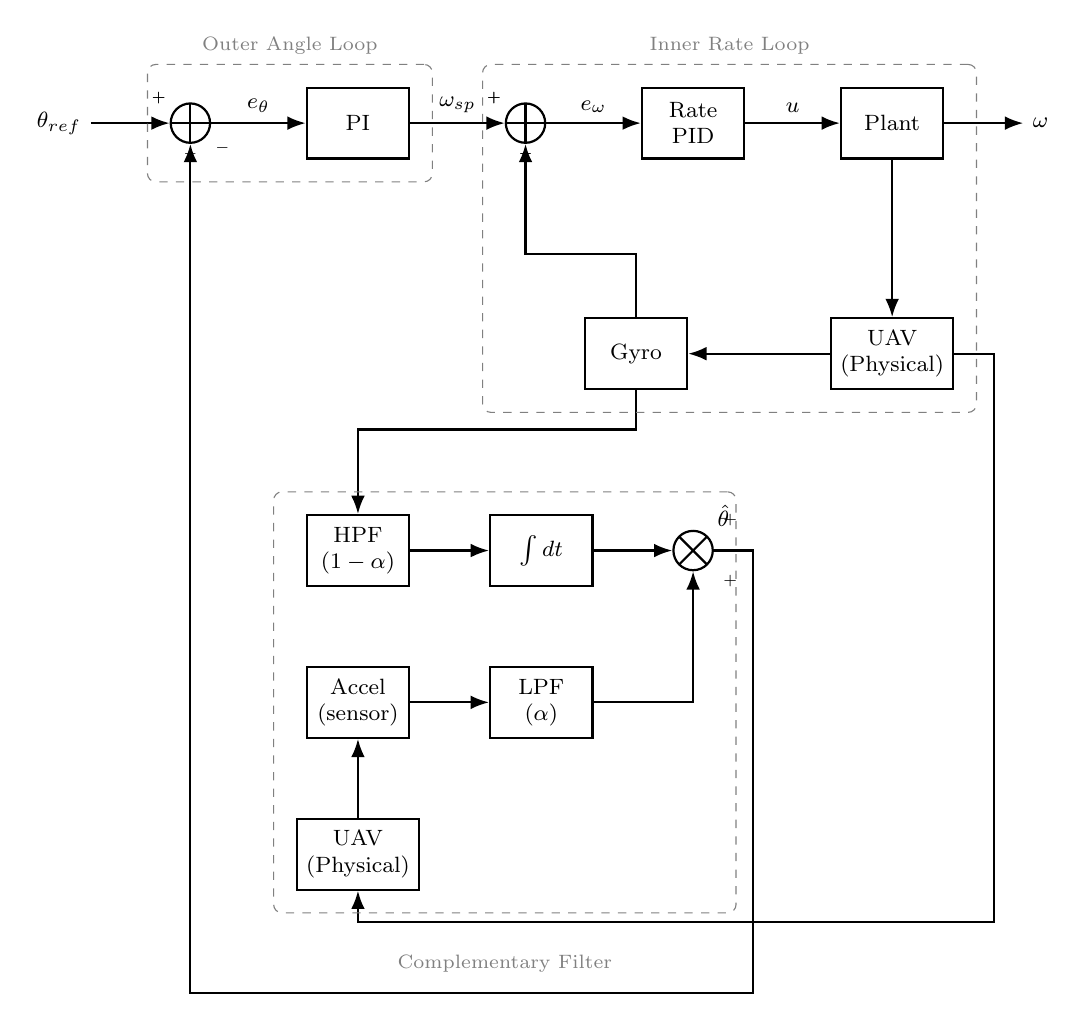
\begin{tikzpicture}[
    node distance = 1.0cm and 1.2cm,
    >=Latex,
    font=\footnotesize,
    block/.style = {draw, rectangle, minimum height=0.9cm, minimum width=1.3cm, align=center, thick},
    sum/.style = {draw, circle, minimum size=0.5cm, thick, path picture={\draw (path picture bounding box.north) -- (path picture bounding box.south) (path picture bounding box.west) -- (path picture bounding box.east);}},
    mixer/.style = {draw, circle, minimum size=0.5cm, thick, path picture={\draw (path picture bounding box.north west) -- (path picture bounding box.south east) (path picture bounding box.north east) -- (path picture bounding box.south west);}},
    group/.style = {draw, dashed, inner sep=8pt, gray, rounded corners=3pt},
    arrow/.style = {->, thick}
]

% =========================================================
% TOP ROW: Main Forward Path (spaced out to avoid overlap)
% =========================================================
\node (theta) {$\theta_{ref}$};
\node[sum, right=1.0cm of theta] (s1) {};
\node[block, right=1.2cm of s1] (pi) {PI};
\node[sum, right=1.2cm of pi] (s2) {};
\node[block, right=1.2cm of s2] (pid) {Rate\\PID};
\node[block, right=1.2cm of pid] (plant) {Plant};
\node[right=1.0cm of plant] (omega) {$\omega$};

% =========================================================
% MIDDLE ROW: Aircraft & Gyro (shifted down more)
% =========================================================
\node[block, below=2.0cm of plant] (air) {UAV\\(Physical)};
\node[block, left=1.8cm of air] (gyro) {Gyro};

% =========================================================
% BOTTOM SECTION: COMPLEMENTARY FILTER
% Positioned below with enough vertical space
% =========================================================

% HPF aligned under the PI block area
\node[block, below=4.5cm of pi] (hpf) {HPF\\$(1-\alpha)$};
\node[block, right=1.0cm of hpf] (int) {$\int dt$};
\node[mixer, right=1.0cm of int] (fuse) {};
\node[below right=0pt and 2pt of fuse] {\tiny +};
\node[above right=0pt and 2pt of fuse] {\tiny +};

% Accel and LPF below HPF
\node[block, below=1.0cm of hpf] (acc) {Accel\\(sensor)};
\node[block, right=1.0cm of acc] (lpf) {LPF\\$(\alpha)$};

% Aircraft source for Accel (at bottom)
\node[block, below=1.0cm of acc] (air2) {UAV\\(Physical)};

% =========================================================
% WIRING: FORWARD PATH
% =========================================================
\draw[arrow] (theta) -- (s1);
\draw[arrow] (s1) -- node[above]{$e_\theta$} (pi);
\draw[arrow] (pi) -- node[above]{$\omega_{sp}$} (s2);
\draw[arrow] (s2) -- node[above]{$e_\omega$} (pid);
\draw[arrow] (pid) -- node[above]{$u$} (plant);
\draw[arrow] (plant) -- (omega);

% Signs for S1 (angle summing junction)
\node[above left=-2pt and 0pt of s1] {\tiny +};
\node[below=-2pt of s1] {\tiny $-$};

% Signs for S2 (rate summing junction)
\node[above left=-2pt and 0pt of s2] {\tiny +};
\node[below=-2pt of s2] {\tiny $-$};

% =========================================================
% WIRING: INNER RATE LOOP
% =========================================================
% Plant to Aircraft
\draw[arrow] (plant.south) -- (air.north);

% Aircraft to Gyro
\draw[arrow] (air.west) -- (gyro.east);

% Gyro feedback to S2
\draw[arrow] (gyro.north) -- ++(0, 0.8) -| (s2.south);

% =========================================================
% WIRING: GYRO TO COMPLEMENTARY FILTER
% =========================================================
\coordinate (gyro_down) at ($(gyro.south) + (0, -0.5)$);
\draw[arrow] (gyro.south) -- (gyro_down) -- (gyro_down -| hpf.north) -- (hpf.north);

% =========================================================
% WIRING: AIRCRAFT TO ACCEL - RE-ROUTED TO FAR RIGHT
% Route: Air -> Right -> Down (past everything) -> Left -> Up to Air2
% This avoids crossing HPF/Accel blocks completely
% =========================================================
\draw[arrow] (air.east) -- ++(0.5, 0) coordinate(air_out)
             -- (air_out |- air2.south) -- ++(0, -0.4) coordinate(air_bottom)
             -- (air_bottom -| air2.south) -- (air2.south);

% Connect Air2 to Accel
\draw[arrow] (air2.north) -- (acc.south);


% =========================================================
% WIRING: COMPLEMENTARY FILTER INTERNAL (Left-to-Right)
% =========================================================
\draw[arrow] (hpf.east) -- (int.west);
\draw[arrow] (int.east) -- (fuse.west);
\draw[arrow] (acc.east) -- (lpf.west);
\draw[arrow] (lpf.east) -| (fuse.south);

% =========================================================
% WIRING: THETA HAT OUTPUT FROM FUSE
% =========================================================
\node[above right=0cm of fuse] (that_label) {$\hat{\theta}$};

% =========================================================
% WIRING: OUTER ANGLE LOOP FEEDBACK
% Route UNDER to avoid crossing sensor input lines
% =========================================================
% From Fuse go Right, then Down past Air2 line, then Left to start, then Up to S1
\draw[arrow] (fuse.east) -- ++(0.5, 0) coordinate(fb_r)
             -- (fb_r |- air2.south) -- ++(0, -1.3) coordinate(fb_bottom)
             -- (fb_bottom -| s1.south) coordinate(fb_corner)
             -- (s1.south);

% Signs for S1 (angle summing junction) - Moved minus sign
\node[above left=-2pt and 0pt of s1] {\tiny +};
\node[below right=-2pt and 0pt of s1] {\tiny $-$};

% Signs for S2 (rate summing junction)
\node[above left=-2pt and 0pt of s2] {\tiny +};
\node[below=-2pt of s2] {\tiny $-$};


% =========================================================
% GROUPS (dashed boxes)
% =========================================================
\node[group, fit=(s1)(pi), label={[gray, font=\scriptsize]above:Outer Angle Loop}] {};
\node[group, fit=(s2)(pid)(plant)(air)(gyro), label={[gray, font=\scriptsize]above:Inner Rate Loop}] {};
\node[group, fit=(hpf)(int)(fuse)(acc)(lpf)(air2), label={[gray, font=\scriptsize, yshift=-0.4cm]below:Complementary Filter}] {};

\end{tikzpicture}
\end{document}
